\section{Motivation}
Das Thema wurde gewählt, weil zelluläre Automaten Teil des wahlobligatorischen Mathematikunterrichts waren. Dort wurde im Lernbereich der Chaostheorie die unten beschriebene "Langton's Ant" \cite{langtonsant} kurz behandelt. Diese stellt jedoch einen einfachen Sonderfall dar. 

Ziel dieser praktischen Umsetzung der Theorie des Unterrichts ist die Simulation von allgemeinen Turmites. Dafür muss dem Benutzer erlaubt werden, das Verhalten beziehungsweise die Regeln der Turmites zu definieren. Das Programm soll als Möglichkeit dienen, den gelernten Stoff aus dem Unterricht zu vertiefen, festigen und erweitern. Dabei wird eine gewisse Grundkenntnis der zugrundeliegenden Theorie vorausgesetzt.

Als Besonderheit soll die Simulation mehrerer Turmites gleichzeitig möglich sein. Dies erfordert eine Erweiterung der Theorie, da die Turmites nacheinander agieren und sich gegenseitig beeinflussen. Letzteres ist besonders interessant, weil aus der Interaktion mehrerer Turmites mit potentiell verschiedenen Regeln neues Verhalten entstehen kann.

\begin{figure}[!htb]
    \minipage{0.32\textwidth}
      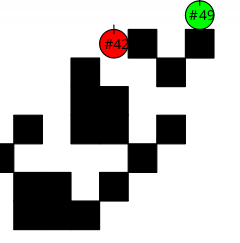
\includegraphics[width=\linewidth]{one.png}
    \endminipage\hfill
    \minipage{0.32\textwidth}
      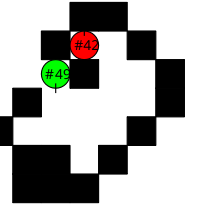
\includegraphics[width=\linewidth]{two.png}
    \endminipage\hfill
    \minipage{0.32\textwidth}%
      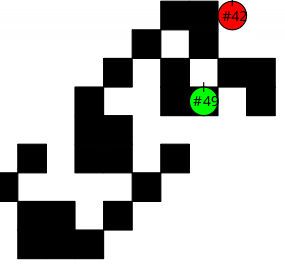
\includegraphics[width=\linewidth]{three.png}
    \endminipage

    \caption{Zwei gespiegelt agierende "Langton's Ants" erzeugen zusammen eine "Linie".}
\end{figure}


\section{Turmites}
Turmites sind zelluläre Automaten. Dabei handelt es sich um "Maschinen", die, einer Übergangstabelle folgend, sich auf einem unendlichen Quadratgitter bewegen. \cite{turmites} Sie besitzen jeweils eine Position, Blickrichtung sowie einen Zustand. Für die Simulation ist eine fortlaufende Iteration notwendig. Dabei wird wie folgt vorgegangen:
\begin{enumerate}
    \item Die Turmite liest die Farbe des Feldes, auf dem sie sich befindet.
    \item Anhand der Übergangstabelle entscheidet sie eine neue Zellfarbe und Drehrichtung.
    \item Die Turmite ändert die Farbe des Feldes, auf dem sie sich befindet.
    \item Die Turmite dreht sich anhand der Drehrichtung.
    \item Die Turmite bewegt sich ein Feld in Blickrichtung.
\end{enumerate}

\subsection{Übergangstabelle}
Eine Übergangstabelle legt fest, wie sich die Turmite in Abhängigkeit von der Zellfarbe und dem Zustand verhält. Sie besteht aus fünf Spalten:
\begin{enumerate}
    \item Zellfarbe (gegeben)
    \item Zustand (gegeben)
    \item Drehrichtung
    \item neue Zellfarbe
    \item neuer Zustand
\end{enumerate}

Die Drehrichtung ist dabei nicht absolut, sprich "nach Norden/Osten/...", sondern relativ, zum Beispiel "90° im Uhrzeigersinn" oder "umkehren".

Ein Spezialfall einer Turmite ist die "Langton's Ant". Jeden Iterationsschritt wechselt sie die Farbe, die sich unter ihr befindet, und dreht sich je nach Farbe nach recht oder links. Dabei nutzt sie zwei Zellfarben und keinen Zustand. Die Übergangstabelle sieht wie folgt aus:

\begin{tabular}{|l|l||l|l|l|}
    \textbf{Zellfarbe} & \textbf{Zustand} & \textbf{Drehricht.} & \textbf{neue Zellfarbe} & \textbf{neuer Zustand} \\
    \hline
    0 (schwarz) & 0 & \textit{nach links} & 1 (weiß) & 0 \\
    1 (weiß) & 0 & \textit{nach rechts} & 0 (schwarz) & 0 \\
\end{tabular}
Übergangstabelle der Langton's Ant, übernommen aus \cite{pflichtenheft}
% \label{tab:langton}

\subsection{Mehrere Turmites auf einem Quadratgitter}
Zur Erfüllung des Kannkriteriums Nr. 2 \cite{pflichtenheft} wurde die Software so erweitert, dass mehrere Turmites gleichzeitig auf einem Quadratgitter simuliert werden können. Dabei müssen mehrere Dinge beachtet werden:

\begin{itemize}
    \item Die Reihenfolge der Turmites ist nicht beliebig und muss vor der Simulation klar definiert sein, da die Turmites in jedem Iterationsschritt nacheinander agieren.
    \item Die Zellfarben müssen für alle Turmites gemeinsam festgelegt werden, währen die Zustände sowie der Rest der Übergangstabelle für jede Turmite individuell anpassbar ist.
\end{itemize}

\section{Ergebnisse}
Ergebnis des Projektes ist sowohl das \texttt{turmites}-Python-Modul als auch die grafische Benutzeroberfläche \texttt{main.py} und \texttt{main\_window.*}.

\subsection{Benutzeroberfläche}
Zur besseren Verständlichkeit werden alle Zustände (Zellzustand/Turmite-Zustand) zusätzlich mit einer Farbe repräsentiert. 

Als Sprache des User Interfaces und aller Bezeichner wurde Englisch gewählt, da das Programm so universeller und für mehr Personen zugänglich ist. Auf Einstellbarkeit der Sprache wurde verzichtet, da dies aus Zeitgründen nicht umsetzbar war sowie nicht im Pflichtenheft \cite{pflichtenheft} gefordert wurde.

Es wurde darauf geachtet, Qt-Layouts zu verwenden, um das Skalieren von Benutzeroberflächenelementen beim Verändern der Fenstergröße zu ermöglichen.

\subsubsection{Hauptfenster}

\begin{figure}[!htb]
    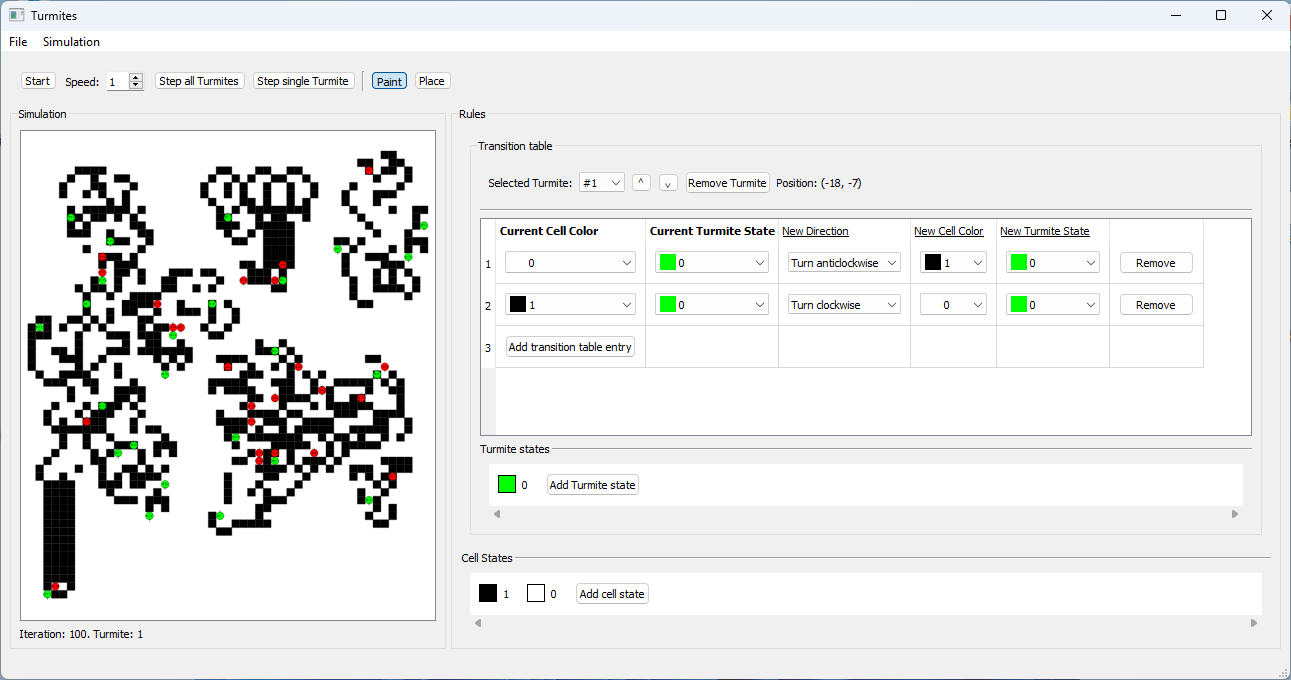
\includegraphics[width=\textwidth]{main_window.png}
    \caption{Hauptfenster}
\end{figure}

In der Werkzeugleiste des Hauptfensters lässt sich die Simulation mit dem "Start"-Knopf starten sowie stoppen. Dieser ändert seine Aufschrift entsprechend. Daneben lässt sich die Simulationsgeschwindigkeit einstellen. Um nur einen Simulationsschritt durchzuführen, kann man entweder den "Step all Turmites"-Knopf betätigen, der eine volle Iteration durchführt, oder den "Step single Turmite"-Knopf betätigen, der nur den Simulationsschritt einer Turmite durchführt. Bei mehreren Turmites erfordert es somit mehrere Klicks letzteren Knopfes, um eine volle Iteration durchzuführen. Es wurden außerdem Tool-Tips zu ausgewählten Knöpfen hinzugefügt, um die Bedienung zu erleichtern.

Der untere Teil des Hauptfensters ist aufgeteilt in Simulationsfläche (Quadratgitter) und Regeleingabe. In der Statusleiste der Simulationsfläche wird die Turmite, die als nächstes agieren wird, zusammen mit der aktuellen Iteration angezeigt. In der Simulationsfläche lässt sich mit Linksklick bewegen und unter Zuhilfenahme des Mausrades zoomen. Per Rechtsklick wird die rechtsseitig in der Werkzeugleiste ausgewählte Aktion durchgeführt ("Place" oder "Paint"). Für die Aktion "Paint" muss zusätzlich eine Zellfarbe in der zugehörigen unten befindlichen Tabelle "Cell states" ausgewählt werden. Die Turmites werden jeweils als ein mit ihrer Nummer beschrifteter Kreis dargestellt, der mit der Farbe des aktuellen Zustandes ausgefüllt ist. Die Blickrichtung gibt ein kleiner Strich an.

Die Regeleingabe ist aufgeteilt in die global, für alle Turmites geltenden Zellfarben und die individuellen Regeln der aktuell ausgewählten Turmite. Diese umfassen Übergangstabelle sowie eine Liste der möglichen Zustände der Turmite. Durch die Knöpfe neben der Turmite-Auswahl lässt sich die aktuell ausgewählte Turmite löschen, soweit sie nicht die einzige ist, sowie die Reihenfolge anpassen. 

\subsubsection{Übergangstabelle}
In der Übergangstabelle lassen sich die einzelnen Anweisungen mittels der Drop-Down-Menüs bearbeiten. Das Hinzufügen und Löschen von Einträgen erfolgt per Knopfdruck. Falls mehrere Anweisungen mit der gleichen Bedingung (beide linken fettgedruckten Spalten) vorhanden sind, ist jeweils nur die neueste gültig und alle anderen werden deaktiviert, bis der Benutzer den Fehler behebt:

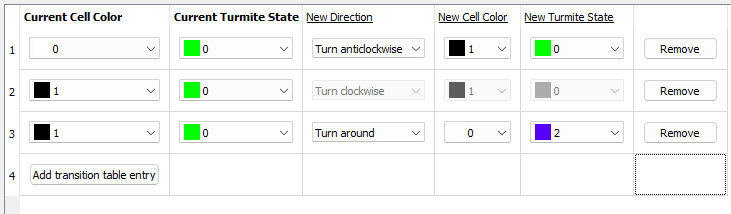
\includegraphics[width=\textwidth]{invalid_table.png}

Falls eine Turmite keine Anweisung für eine bestimmte Bedingung besitzt, wird eine Fehlermeldung angezeigt und die Simulation gestoppt:

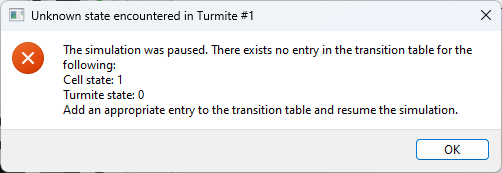
\includegraphics[width=\textwidth]{unknown_state.png}

\subsubsection{Zell- und Turmite-Zustände}
Per Rechtsklick lässt sich die Farbe von Zuständen nachträglich ändern sowie ein Zustand löschen. Per Knopfdruck lässt sich ein neuer Zustand hinzufügen. Die Nummer des neuen Zustandes wird dabei automatisch ergänzt und die Farbe ist durch den Benutzer mittels Farbauswahl auswählbar.

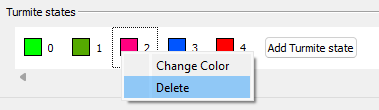
\includegraphics[width=\textwidth]{context_menu_states.png}

\section{Entwicklung}
\subsection{Hilfsmittel}
Zur Entwicklung wurde das Internet intensiv genutzt. Dabei wurden unter Nutzung der Google-Suchmaschine \cite{google} diverse Dokumentationen, zum Beispiel die Qt5-Dokumentation \cite{qt5}, und andere Websites, wie beispielsweise StackOverflow \cite{stackoverflow} zur Hilfe genommen. Außerdem wurde die Software Git \cite{git} sowie die Website GitHub \cite{github} zur Versionsverwaltung genutzt. Für ausgewählte Probleme bezüglich Qt5 und dessen Widgets wurde zusätzlich ChatGPT \cite{chatgpt} genutzt.

\subsection{Architektur}
Bei der Konzipierung der Software wurde auf eine strikte Trennung von Darstellung und Logik geachtet. Die gesamte Kernfunktion der Software befindet sich in einem separaten Python-Modul \texttt{turmites}.

Das Konzept des unendlichen Quadratgitters wurde ebenfalls in einer unabhängigen generischen Klasse \texttt{InfiniteGrid} abstrahiert. Dadurch ist eine Wiederverwendbarkeit und Erweiterbarkeit der Software gewährleistet, zum Beispiel in der Form einer Neuimplementierung einer grafischen Benutzeroberfläche. Auch die Verknüpfung von mehreren Turmites in einem Quadratgitter ist dort implementiert. 

Das einfärben der verschiedenen Zustände ist jedoch in der Darstellung implementiert (\texttt{main.py}), da es sich um eine rein visuelle Eigenschaft handelt. Auch das Konzept eines Projektes (\texttt{Project}) wird dort erst eingeführt.

Generell wurde bei der Entwicklung auf eine möglichst objektorientierte Programmierung geachtet.

Um das Speichern und Öffnen (Serialisierung und Deserialisierung) zu ermöglichen, sind alle relevanten Klassen mit \texttt{to\_json()}- und \texttt{from\_json()}-Methoden ausgestattet. JSON \cite{json} wurde gewählt, da es ein einfaches und menschenlesbares Format ist, was die Implementierung erleichtert. Außerdem ist es in Python bereits integriert.

\subsubsection{"Unendliches" Quadratgitter}
Auch wenn die Simulationsfläche praktisch gesehen endlich ist, da irgendwann jede noch so effiziente Implementierung den Arbeitsspeicher des Computers voll auslastet, wurde darauf geachtet, dass die Speicherauslastung nicht von der Distanz der aktivierten Zelle zu einem Koordinatenursprung abhängt, sondern von der Anzahl an aktivierten Zellen.

Dies wurde umgesetzt unter Zuhilfenahme eines Python-Dictionaries, welches die Koordinaten der aktiven Zellen als Schlüssel und die jeweiligen Zustände als Werte speichert. Dadurch ist die Zugriffszeit auf eine Zelle konstant und unabhängig von der Anzahl an Zellen. Die Speicherauslastung steigt jedoch linear zur Anzahl an Zellen. Im Gegensatz zu einem zweidimensionalen Array, welches die Speicherauslastung quadratisch zur Distanz zum Koordinatenursprung steigen lassen würde, ist dies jedoch ein akzeptabler Kompromiss. Zudem ist es nicht trivial, die Größe eines solchen Arrays dynamisch anzupassen. Außerdem werden nichtaktivierte oder deaktivierte Zellen, sprich Zellen die den Standardwert besitzen, nicht im Dictionary gespeichert, um Speicherplatz zu sparen.

Es folgt ein minimales Beispiel für eine solche Implementierung:

% with font courier
\begin{lstlisting}[language=Python]
    class InfiniteGrid:
        def __init__(self, default: int):
            self._grid: dict[Position, T] = {}
            self.default = default

        def __setitem__(self, key: Position, value: T):
            if value == self.default:
                self._grid.pop(key, None)
            else:
                self._grid[key] = value

        def __getitem__(self, item: Position):
            return self._grid.get(item, self.default)

\end{lstlisting}

\section{Diskussion}
Es wurden alle Muss- und Sollkriterien bis auf folgende Ausnahmen erfüllt:

Die Darstellung \cite[1.2.1]{pflichtenheft} ist zwar "performant[e] und flüssig[e]" genug für den einfachen Gebrauch. Bei längeren Simulationen (mehr aktivierte Zellen) und vielen Turmites kommt es jedoch zu einer Verlangsamung. Die weitere Optimierung der Darstellung wurde aus Zeitgründen nicht weiter verfolgt.

Das gesonderte Speichern der Übergangstabelle (der "Regeln" \cite[1.1.6]{pflichtenheft}) wurde außerdem nicht ermöglicht, da beim Importieren einer Übergangstabelle die Zell- sowie Turmitezustände abgeglichen und überprüft werden müssten sowie hilfreiche Fehlermeldungen bereitgestellt werden sollten. Zudem wurde es nicht ermöglicht, die Simulationsfläche \cite[1.1.6]{pflichtenheft}, zum Beispiel als Bilddatei, zu exportieren. Dies ist mit einem großen Aufwand verbunden, der nicht in die Zeitplanung passte.

\subsection{Benutzeroberfläche}
Der gesamte Code für die Kernlogik umfasst ca. 174 Zeilen \cite{cloc}, während die Datei \texttt{main.py}, welche sich Vordergründig mit der Verwaltung der Benutzeroberfläche befasst, ca. 627 Code-Zeilen \cite{cloc} besitzt. Dies zeigt den Aufwand der Implementierung der Benutzeroberfläche, welche den Großteil der Entwicklungszeit in Anspruch genommen hat, während die Kernlogik innerhalb weniger Stunden implementiert war.

Diese Komplexität stammt unter anderem daher, dass Änderungen während der Simulation erlaubt und sofort übernommen werden sowie dass es viele Grenzfälle gibt, die alle überprüft werden müssen. Ein noch nicht hinreichend behandelter Fall ist das Löschen von Turmite- oder Zellzuständen während einer Simulation, die bereits genutzt werden. Aus Gründen der Softwarearchitektur ist es ohne größere Änderungen nicht möglich, das Löschen beider Zustandsarten separat beziehungsweise anders zu behandeln, da diese in einer abstrahierten Art und Weise implementiert sind.

\subsubsection{Übergangstabelle}
Die Implementierung der Übergangstabelle war sehr aufwendig. Dies liegt mitunter daran, dass es möglich ist, ungültige Übergangstabellen einzugeben, sowie dass die Farben sich automatisch und sofort ändern müssen, wenn der Benutzer diese nachträglich in den Tabellen darunter ändert. Weiterhin wäre es von Vorteil für den Benutzer, wenn beispielsweise fehlende Einträge direkt angezeigt werden, statt erst beim Ausführen der Simulation zu einem Fehler zu führen. Über die Positionierung des Knopfes zum Hinzufügen eines Eintrages lässt sich Diskutieren, da dieser mit der Zeit immer weiter nach unten rutscht.

Generell wäre es eventuell besser gewesen, die Übergangstabelle in Textform einzugeben, statt als Qt-Tabelle mit Drop-Down-Menüs. Dies hätte die Implementierung deutlich vereinfacht, jedoch die Benutzerfreundlichkeit verringert. Das gleichzeitige oder gruppierte Konfigurieren mehrerer Turmites wäre ebenfalls eine sinnvolle Erweiterung.

\subsection{Implementierung}
Das Speicherformat der Simulationsfläche ist verbesserungswürdig. Aktuell werden alle aktivierten Zellen in einer Liste in Textform gespeichert. Eine binäres Speicherformat wäre effizienter.  

Das Testen der Applikation ist unzulänglich erfolgt, weshalb viele noch nicht betrachtete Grenzfälle existieren und, wenn ausgelöst, das Programm zum Absturz bringen. Zudem wurde das Programm auch auf anderen Betriebssystemen wie Linux und MacOS getestet, jeweils mit bestimmten Problemen, die auf Windows nicht auftreten. Deshalb wurde die Behebung dieser Fehler auch nicht weiter verfolgt.

Generell folgt der Programmcode der \texttt{main.py} nur begrenzt den best practices und Vorgaben der objektorientierten Programmierung wie zum Beispiel der separation of concerns \cite{separationofconcerns}. 